
%(BEGIN_QUESTION)
% Copyright 2014, Tony R. Kuphaldt, released under the Creative Commons Attribution License (v 1.0)
% This means you may do almost anything with this work of mine, so long as you give me proper credit

Beregn utgangsspenningene fra disse to spenningsdelerkretsene ($V_A$ og $V_B$):

$$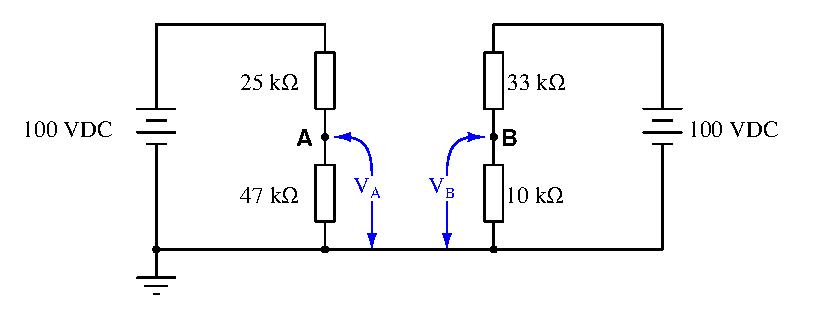
\includegraphics[width=15.5cm]{i01238x01.eps}$$

Beregn deretter spenningen mellom punkt {\bf A} (rød måleledning) og punkt {\bf B} (svart måleledning), altså $V_{AB}$.

\underbar{file i01238}
%(END_QUESTION)





%(BEGIN_ANSWER)

$V_A =$ + 65.28 V

\vskip 10pt

$V_B =$ + 23.26 V

\vskip 10pt

$V_{AB} =$ + 42.02 V (punkt {\bf A} er positivt i forhold til punkt {\bf B})

%(END_ANSWER)





%(BEGIN_NOTES)


%INDEX% Elektronikkrepetisjon: serie- og parallellkretser

%(END_NOTES)

